\documentclass[a4paper,11pt]{article}

\usepackage{graphicx} % Required for inserting images
\usepackage[english,greek]{babel}
\usepackage[utf8x]{inputenc}
\usepackage{amsmath}
\usepackage{multirow}
\usepackage{enumitem}
\usepackage{graphicx}
\usepackage{subcaption}
\usepackage{float}
\usepackage{array}
\usepackage{changepage}
\usepackage[nottoc]{tocbibind}


\graphicspath{images/}

\newcommand{\lt}{\latintext}
\newcommand{\gt}{\greektext}

\setlength{\arrayrulewidth}{0.3mm}
\setlength{\tabcolsep}{8pt}
\renewcommand{\arraystretch}{1.5}

\title{Πρώτη υποχρεωτική εργασία στην Αριθμητική Ανάλυση}
\author{\gt Ονοματεπώνυμο: Νικόλαος Αργυρίου \\  ΑΕΜ: 4367}
\date{\today}

\begin{document}

\maketitle

\section{Άσκηση 1}
\subsection{Εισαγωγή}

Ο κώδικας για την άσκηση βρίσκεται στο αρχείο \lt ask1.py. \gt Αρχικά ορίζουμε τη συνάρτηση \lt \(f(x) = 14xe^{x-2}-12e^{x-2}-7x^3+20x^2-26x+12\), \gt η οποία εμφανίζεται στο σχήμα \ref{fig:1_1}.

\begin{figure}[h!]
    \centering
    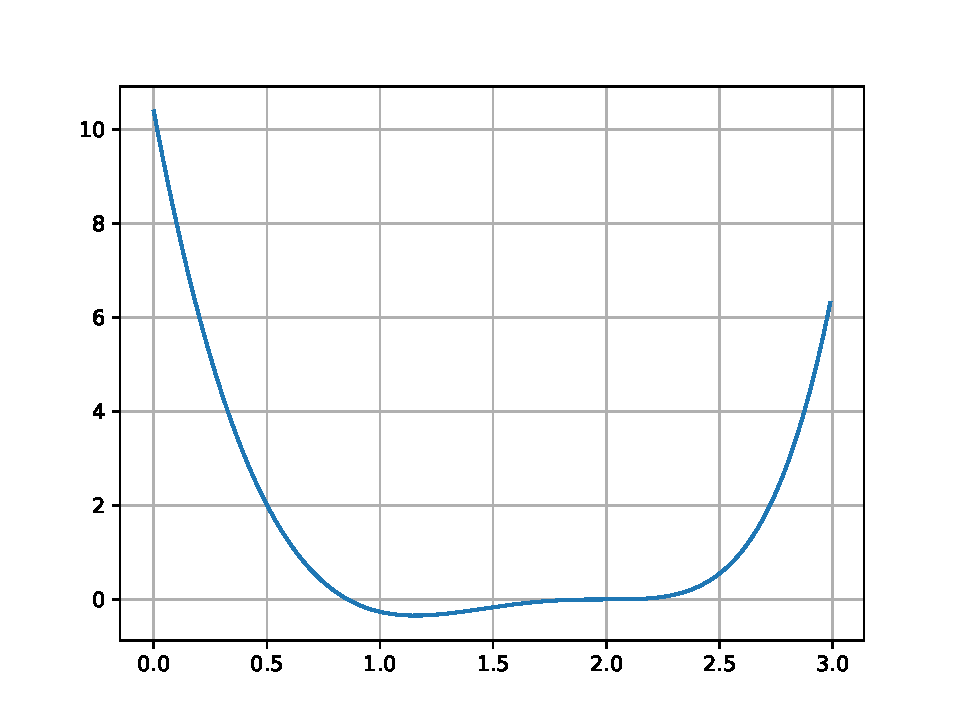
\includegraphics[width=0.8\linewidth]{images/ask1_1.pdf}
    \centering
     \caption{Η γραφική παράσταση της \lt \(f(x)\) \gt στο διάστημα \([0, 3]\)}
    \label{fig:1_1}
\end{figure}

Εάν εστιάσουμε στο διάστημα \([0.5, 2.5]\), όπως φαίνεται στο σχήμα \ref{fig:1_2}, παρατηρούμε ότι η συνάρτηση έχει δύο ρίζες. Πράγματι εφαρμόζοντας διαδοχικά το θεώρημα \lt Bolzano \gt στα διαστήματα \([0, 1]\) και \([1, 3]\) και παρατηρώντας ότι η συνάρτηση είναι γνησίως μονότονη σε καθένα από αυτά συμπεραίνουμε ότι η \lt \(f\) \gt έχει ακριβώς μία ρίζα στο \([0, 1]\) και ακριβώς μία ακόμα στο \([1, 3]\). Σε αυτά τα διαστήματα θα εφαρμόσουμε τη μέθοδο της διχοτόμησης.

\begin{figure}[h!]
\centering
    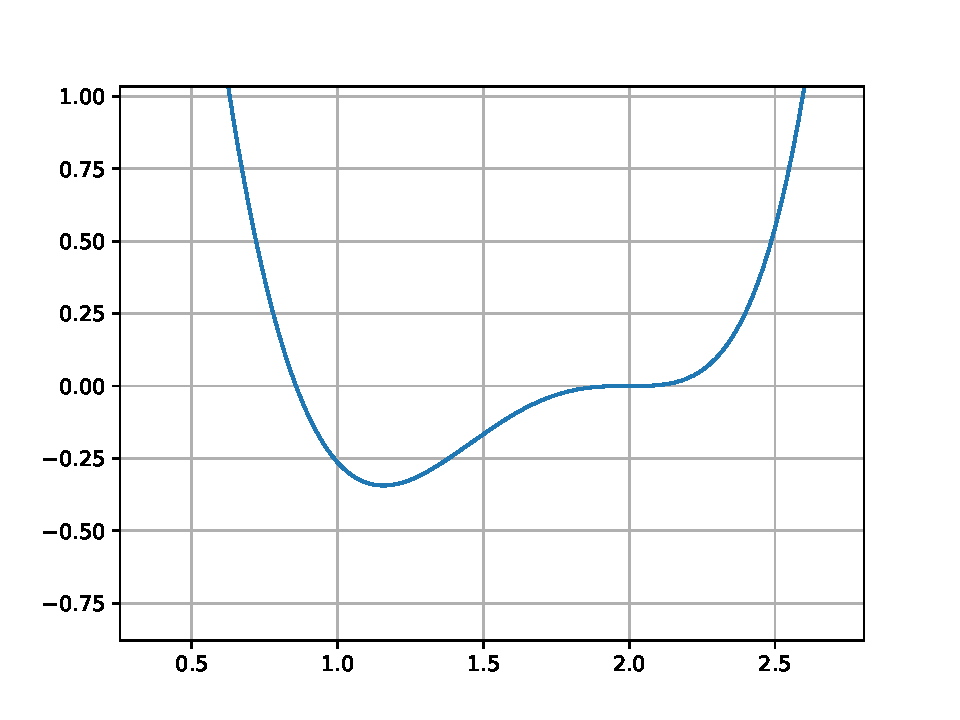
\includegraphics[width=0.8\linewidth]{images/ask1_2.pdf}
    \centering
    \caption{Η γραφική παράσταση της \lt \(f(x)\) \gt στο διάστημα \([0.5, 2.5]\)}
    \label{fig:1_2}
\end{figure}

\subsection{Μέθοδος της διχοτόμησης}

% Στην αρχή υπολογίζουμε τον αριθμό των βημάτων N που απαιτούνται ώστε να έχουμε ακρίβεια 5 δεκαδικών στοιχείων με τη βοήθεια του τύπου 

% \begin{displaymath}
%     \centering
%     \frac{b-a}{2^N}<0.5*10^{-5} => N>\log_2(\frac{b-a}{5}10^{6})
% \end{displaymath}

Εκτελούμε τον αλγόριθμο της διχοτόμησης. Η μικρότερη υπολογισμένη ρίζα είναι η 0.8571395874023438, η οποία χρειάστηκε 17 βήματα εκτέλεσης και η μεγαλύτερη είναι η 2.0 με 1 βήμα εκτέλεσης.

% \newpage

\subsection{Μέθοδος \lt Newton-Raphson}

\gt Αρχικά ας υπολογίσουμε τις παραγώγους της συνάρτησης $f$:

\begin{displaymath}
    f'(x) = 2e^{x-2}(7x+1)-21x^2+40x-26
\end{displaymath}
\begin{displaymath}
    f''(x) = 2e^{x-2}(7x+8)-42x+40
\end{displaymath}
\begin{displaymath}
    f^{(3)}(x) = 2e^{x-2}(7x+15)-42
\end{displaymath}

Οι γραφικές παραστάσεις των δύο πρώτων παρουσιάζονται στο σχήμα \ref{fig:1_3}.

\begin{figure}[H]
    \centering
    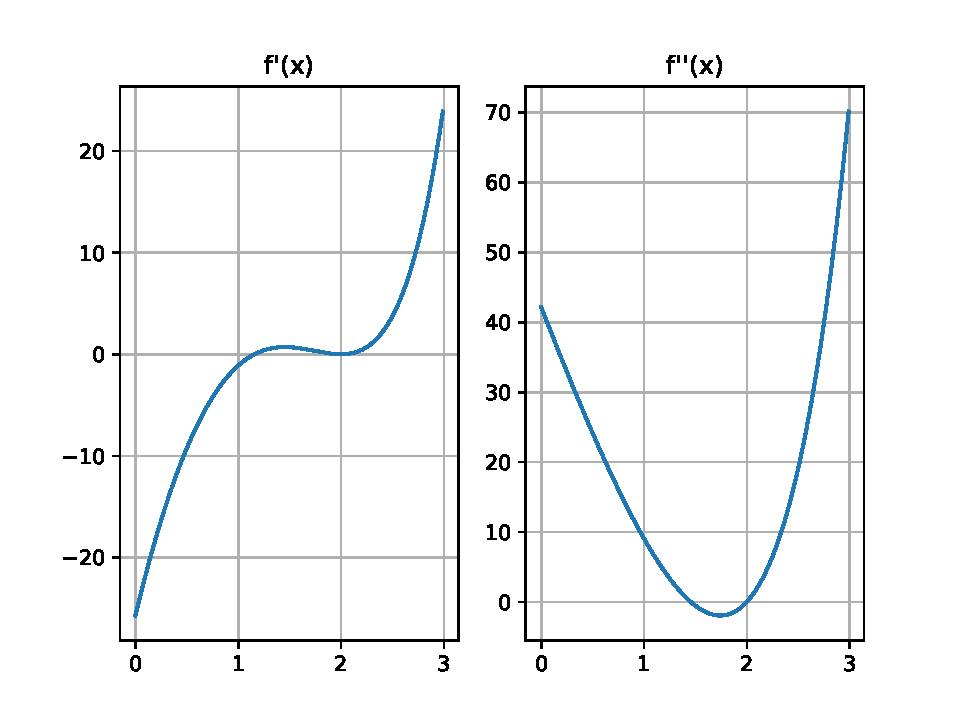
\includegraphics[width=0.8\linewidth]{images/ask1_3.pdf}
    \caption{\gt Η γραφική παράσταση των \lt \(f'(x)\) \gt και \lt \(f''(x)\) \gt στο διάστημα \([0, 3]\)}
    \label{fig:1_3}
\end{figure}

Όσον αφορά τη μικρότερη ρίζα, επιλέγουμε ως αρχικό σημείο για τον αλγόριθμο το $x_0 = 0$, καθώς επαληθέυεται η σχέση $f(0)f''(0)>0$, όπως εύκολα διαπιστώνουμε από τα σχήματα \ref{fig:1_1} και \ref{fig:1_3}. Η υπολογισμένη ρίζα είναι η 0.8571428571428563 και χρειάστηκαν 7 βήματα του αλγορίθμου για τον υπολογισμό της, επομένως η σύγκλιση είναι τετραγωνική.

Εκτελώντας τον αλγόριθμο για τη μεγαλύτερη ρίζα έχουμε $r =$ \\ 2.000008211456383 και παρατηρούμε ότι η σύγκλιση γίνεται γραμμική, εφόσον τα βήματα εκτέλεσης είναι 29. Αυτό φαίνεται και από το γεγονός ότι \(f'(2)=f''(2)=0\) και \(f^{(3)}(2)=16\), δηλαδή ότι η ρίζα αυτή είναι πολλαπλότητας 3 που είναι μεγαλύτερη του 1. Για να αντιμετωπίσουμε αυτό το πρόβλημα εφάρμοζουμε την παραλλαγή της μεθόδου \lt Newton-Raphson. \gt Έτσι λαμβάνουμε την εκτιμώμενη ρίζα 2.000000407109992 με 6 βήματα εκτέλεσης.

\subsection{Μέθοδος της τέμνουσας}

Με αρχικά σημεία τα $x_0=0$ και $x_1=1$ ο αλγόριθμος μάς επιστρέφει τη ρίζα 0.8571428579150075 σε 7 επαναλήψεις. Θέτοντας τώρα $x_0=1$ και $x_1=3$ λαμβάνουμε πάλι προσέγγιση της προηγούμενης ρίζας. Αν όμως μεταφέρουμε τα αρχικά πιο κοντά στη μεγαλύτερη ρίζα, δηλαδή θέτοντας $x_0=1.5$ και $x_1=2.5$ λάμβάνουμε την προσέγγιση 1.9999825845066377 σε 35 βήματα εκτέλεσης.

\subsection{Συμπεράσματα}

\begin{table}[h]
    \centering
    \caption{Σύγκριση των τριών μεθόδων}
    \label{fig:1_4}
    \makebox[\textwidth]{
        \begin{tabular}{c >{\centering\arraybackslash}m{10em} >{\centering\arraybackslash}m{10em} >{\centering\arraybackslash}m{10em}}
            \hline
            & Μέθοδος διχοτόμησης & \lt Newton-Raphson & \gt Μέθοδος τέμνουσας \\
            \hline
            Μικρή ρίζα & 0.8571395874023438 & 0.8571428571428563 & 0.8571428579150075 \\
            Βήματα εκτέλεσης & 17 & 7 & 7 \\
            \hline
            Μεγάλη ρίζα & 2.0 & 2.000000407109992 & 1.9999825845066377 \\
            Βήματα εκτέλεσης & 1 & 6 & 35 \\
            \hline
        \end{tabular}
    }
\end{table}

Στον πίνακα \ref{fig:1_4} συγκρίνονται η τρεις μέθοδοι ως προς τις προσεγγίσεις των ριζών και πόσες επαναλήψεις χρειάστηκαν για τη σύγκλιση. Για τη μικρότερη ρίζα τη πρωτιά μοιράζονται οι μέθοδοι \lt Newton-Raphson \gt και τέμνουσας, ενώ αυτή της διχοτόμησης καθίσταται πιο αργή. Ωστόσο τα αποτελέσματα ανατρέπονται όσον αφορά τη μεγαλύτερη ρίζα. Η μάθοδος της διχοτόμησης είναι η γρηγορότερη με μόνο μία επανάληψη! Ακολουθούν οι μέθοδοι \lt Newton-Raphson \gt και της τέμνουσας.

\section{Άσκηση 2}

Ο κώδικας για την άσκηση βρίσκεται στο αρχείο \lt ask2.py. \gt

\subsection{} %2.1

\begin{figure}[H]
\centering
    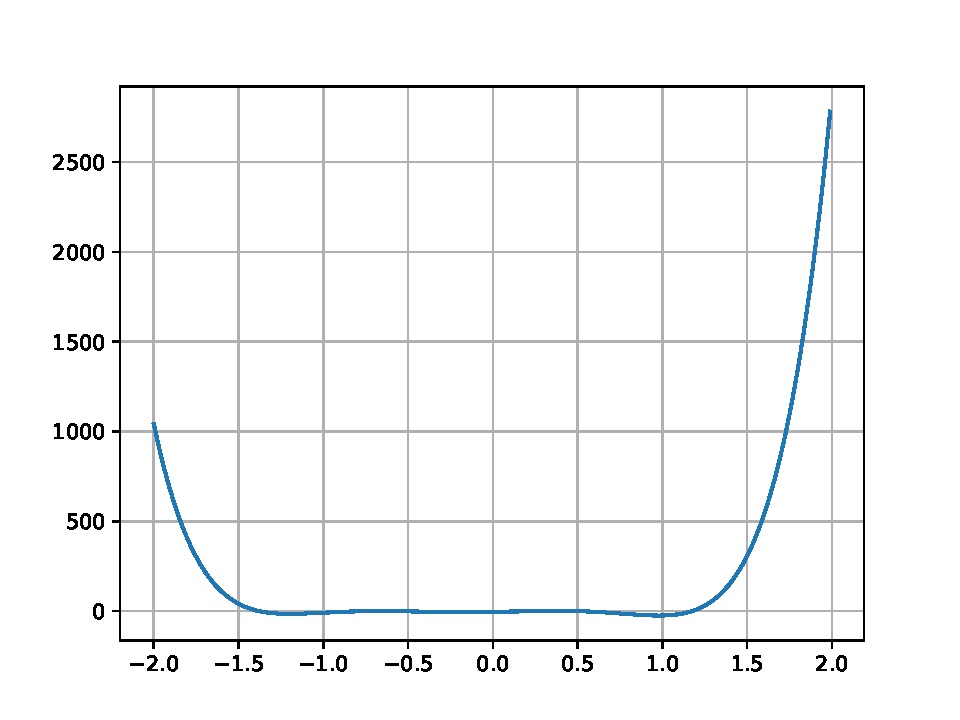
\includegraphics[width=0.8\linewidth]{images/ask2_1.pdf}
    \centering
    \caption{Η γραφική παράσταση της \lt \(f(x)\) \gt στο διάστημα \([-2, 2]\)}
    \label{fig:2_1}
\end{figure}

\begin{figure}[H]
\centering
    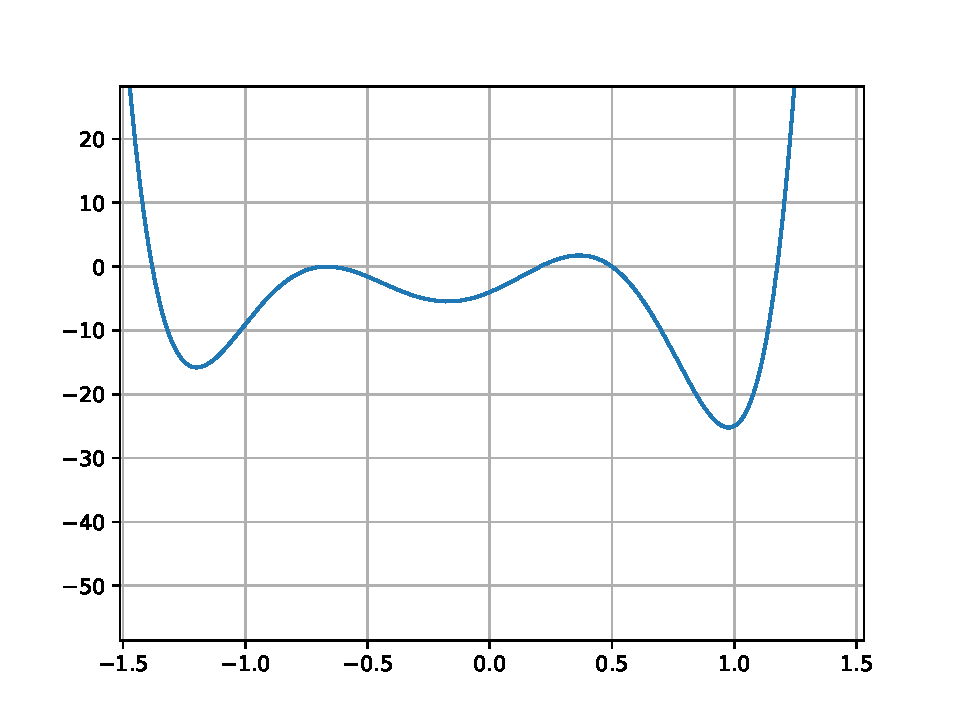
\includegraphics[width=0.8\linewidth]{images/ask2_2.pdf}
    \centering
    \caption{Η γραφική παράσταση της \lt \(f(x)\) \gt από πιο κοντά}
    \label{fig:2_2}
\end{figure}

Με βάση τα σχήματα \ref{fig:2_1} και \ref{fig:2_2} γίνεται η επιλογή των αρχικών σημείων για την εκτέλεση των τριών μεθόδων.

\begin{table}[h]
\centering
\caption{Αποτελέσματα της τροποποιημένης μεθόδου \lt Newton-Raphson}
\label{fig:2_3}
\begin{tabular}{c c c}
    \gt Ρίζα & Βήματα & Αρχική τιμή \\ \hline
    -1.3812984820439949 & 5 & -2 \\
    -0.6666675118200035 & 12 & -1 \\
    0.20518292468904759 & 3 & 0.13 \\
    0.5 & 4 & 0.7 \\
    1.176115557354947 & 5 & 2 \\
\end{tabular}
\end{table}


\begin{table}[h]
\centering
\caption{Αποτελέσματα της τροποποιημένης μεθόδου διχοτόμησης}
\label{fig:2_4}
\begin{tabular}{c c c c}
    \gt Ρίζα & Βήματα & \lt a & \lt b  \\ \hline
    -1.3812969988250796 & 20 & -1.6 & -1.2 \\
    0.20518062506125279 & 28 & 0 & 0.4 \\
    0.5000026907141163 & 19 & 0.3 & 0.7 \\
    1.1761160666642803 & 20 & 1 & 1.4 \\
\end{tabular}
\end{table}


\begin{table}[h]
\centering
\caption{\gt Αποτελέσματα της τροποποιημένης μεθόδου τέμνουσας}
\label{fig:2_5}
\begin{tabular}{c c c c c}
    \gt Ρίζα & Βήματα & $x_0$ & $x_1$ & $x_2$ \\ \hline
    -1.3812984820439953 & 6 & -1.6 & -1.4 & -1.2 \\
    -0.666662589750732 & 19 & -0.8 & -0.6 & -0.4 \\
    0.20518292468904759 & 5 & 0 & 0.2 & 0.4 \\
    0.5000000000000191 & 12 & 0.3 & 0.4 & 0.7 \\
    1.17611555735478 & 5 & 1 & 1.2 & 1.4 \\
\end{tabular}
\end{table}

Στους πίνακες \ref{fig:2_3}, \ref{fig:2_4} και \ref{fig:2_5} παρουσιάζονται τα αποτελέσματα της εκτέλεσης των αλγορίθμων. Από την τροποποιημένη μέθοδο διχοτόμησης λείπει η δεύτερη ρίζα, καθώς δεν ισχύει το θεώρημα \lt Bolzano \gt σε κάποιο κοντινό της διάστημα. Επίσης αξίζει να σημειωθεί εδώ ότι η συνθήκη τερματισμού της τροποποιημένης μεθόδου διχοτόμησης είναι η \(b-a < tolerance\), αντί για την \(\frac{b-a}{2} < tolerance\), όπου $a$ και $b$ τα άκρα του διαστήματος σε δεδομένο βήμα εκτέλεσης του αλγορίθμου, καθώς πλέον η υπολογιζόμενη ρίζα μπορεί να βρίσκεται σε οποιοδήποτε σημείο του διαστήματος \(\left[ a, b\right]\) και όχι αναγκαστηκά στο μέσο του. 

\subsection{} %2.2

Τρέχοντας τον αλγόριθμο της τροποιημένης μεθόδου διχοτόμησης 20 φορές παρατηρούμε ότι δεν συγκλίνει πάντα στον ίδιο αριθμό επαναλήψεων, αλλά ο αριθμός τους διαφέρει κάθε φορά: [26, 19, 20, 23, 17, 22, 24, 30, 31, 20, 19, 31, 27, 29, 26, 23, 15, 18, 31, 23]. Αυτό είναι λογικό αν λάβουμε υπόψη την χρήση της συνάρτησης τυχαίων αριθμών.

\subsection{} %2.3

\begin{table}[h]
    \centering
    \caption{Σύγκριση των μεθόδων για κάθε ρίζα}
    \label{fig:2_6}
    \makebox[\textwidth]{
        \begin{tabular}{c c c c c c}
            & 1η & 2η & 3η & 4η & 5η \\
            \hline
            Τροποποιημένη \lt Newton-Raphson & 5 & 12 & 3 & 4 & 5 \\
            Κλασσική \lt Newton-Raphson & 8 & 16 & 4 & 5 & 8 \\
            \hline
            Τροποποιημένη διχοτόμηση & 20 & - & 28 & 19 & 20 \\
            Κλασσική διχοτόμηση & 16 & - & 16 & 1 & 16 \\
            \hline
            Τροποποιημένη τέμνουσα & 6 & 19 & 5 & 12 & 5 \\
            Κλασσική τέμνουσα & 12 & 9 & 6 & 15 & 9 \\
        \end{tabular}
    }
\end{table}

Μελετώντας τον πίνακα \ref{fig:2_6} παρατηρούμε ότι η τροποιημένη μέθοδος \lt Newton-Raphson \gt είναι αρκετά γρηγορότερη της αντίστοιχης κλασσικής. Το ίδιο ισχύει και για την τροποποιημένη μέθοδο τέμνουσας, αν εξαιρέσουμε την περίπτωση της δεύτερης ρίζας. Όμως η κλασσική μέθοδος διχοτόμησης φαίνεται να είναι γενικά γρηγορότερη της τροποποιημένης, αλλά αυτό εξαρτάται από τις τιμές που επιστρέφει κάθε φορά η συνάρτηση παραγωγής ψευδοτυχαίων αριθμών.

\section{Άσκηση 3}

Ο κώδικας για την άσκηση βρίσκεται στο αρχείο \lt ask3.py. \gt

\subsection{Επίλυση γραμμικών συστημάτων με τη μέθοδο \lt PA=LU}

\gt Η συνάρτηση που υλοποιεί αυτήν τη μέθοδο είναι η \lt \verb|solve_system|. \gt Λαμαβάνει ως είσοδο έναν πίνακα συντελεστών $Α$ και το διάνυσμα \lt $b$, \gt τα οποία προέρχονται από τη σχέση \(Ax = b\) και επιστρέφει το υπολογισμένο διάνυσμα λύσεων $x$. Αρχικά υπόλογίζεται η παραγοντοποίηση \lt PA=LU \gt του πίνακα $Α$ μέσω της συνάρτησης \lt \verb|palu|, \gt η οποία με τη σειρά της χρησιμοποιεί τη συνάρτηση \lt \verb|place_max_to_pivot| \gt για να κάνει τις απαραίτητες αντιμεταθέσεις γραμμών του πίνακα, ώστε κάθε φορά το οδηγό στοιχείο να έχει τη μεγαλύτερη απόλυτη τιμή στη στήλη του.

\subsection{Αποσύνθεση \lt Cholesky}

\gt Η συνάρτηση που υλοποιεί την αποσύνθεση \lt Cholesky \gt είναι η \lt \verb|cholesky|, \gt η οποία δέχεται έναν συμμετρικό και θετικά ορισμένο πίνακα $A$ και επιστρέφει τον κάτω τριγωνικό πίνακα $L$.

\subsection{Μέθοδος \lt Gauss-Seidel}

\gt Η συνάρτηση που υλοποιεί τη μέθοδο \lt Gauss-Seidel \gt είναι η \lt \verb|gauss_seidel|, \gt η οποία δέχεται έναν τετραγωνικό πίνακα $A$, ένα διάνυσμα $b$, μία αρχική εκτίμηση της λύσης $χ_0$ και την ανοχή του σφάλματος και επιστρέφει το διάνυσμα των λύσεων $x$, ώστε να ικανοποιείται η εξίσωση $Ax=b$.

Οι πίνακες $Α$ των δύο γραμμικών συστημάτων έχουν κυριαρχική διαγώνιο, συνεπώς η μέθοδος \lt Gauss-Seidel \gt συγκλίνει. Επιλέγουμε ως αρχικό διάνυσμα το μηδενικό. Λύνοντας το \lt 10x10 \gt σύστημα λαμβάνουμε την εκτιμώμενη λύση 
\begin{align*}
   x &= [0.99995742, 0.99993697, 0.99993202, 0.99993688, \\ &\qquad0.99994706, 0.99995922, 0.99997116, 0.99998158,\\ &\qquad0.99998988, 0.99999595]^{T}
\end{align*}

Λύνοντας τώρα το \lt 10000x10000 \gt σύστημα λαμβάνουμε μετά από μερικά λεπτά την εκτιμώμενη λύση
\begin{align*}
    x &= [1.00094083, 1.00238244, 1.0050532,  \cdots 0.87499504, 0.74999732, 0.49999893]^{T}
\end{align*}

\section{Άσκηση 4}

Ο κώδικας για την άσκηση βρίσκεται στο αρχείο \lt ask4.py. \gt

\subsection{} % 4.1

Θα υπολογίσουμε το άθροισμα των στοιχείων μιας τυχαίας στήλης \lt j \gt του πίνακα \lt \textbf{G}:

\[\sum_{i=1}^{n}\boldsymbol{G}_{(i,j)} = \sum_{i=1}^{n}\bigg(\frac{q}{n}+\frac{A_{(j,i)}(1-q)}{n_j}\bigg) =\] \[\sum_{i=1}^{n}\frac{q}{n} + \sum_{i=1}^{n}\frac{A_{(j,i)}(1-q)}{n_j} = n\frac{q}{n} + \frac{1-q}{n_j}\sum_{i=1}^{n}A_{(j,i)}\]

\gt Όμως το τελευταίο άθροισμα ουσιαστικά προσθέτει όλα τα στοιχεία της γραμμής \lt j \gt του πίνακα \lt \textbf{A}. \gt Συνεπώς \(\sum_{i=1}^{n}A_{(j,i)} = n_j\). Οπότε έχουμε:

\[n\frac{q}{n} + \frac{1-q}{n_j}\sum_{i=1}^{n}A_{(j,i)} = q + \frac{1-q}{n_j}n_j = q+1-q = 1\]

Έτσι δείξαμε ότι μία οποιαδήποτε τυχαία στήλη του πίνακα \lt \textbf{G} \gt δίνει άθροισμα 1 που σημαίνει ότι ο πίνακας είναι στοχαστικός.

\subsection{} % 4.2

\gt Αρχικά μεταφέρουμε τον πίνακα Α στο αρχείο με τον κώδικα. Στη συνέχεια χρησιμοποιώντας τη συνάρτηση \lt \verb|get_google| \gt υπολογίζουμε τον πίνακα $\boldsymbol{G}$ με βάση τον τύπο:

\[\boldsymbol{G}_{(i,j)} = \frac{q}{n} + \frac{\boldsymbol{A}_{(j,i)}(1-q)}{n_j}\]

Για τον υπολογισμό της μέγιστης ιδιοτιμής και του αντίστοιχου ιδιοδιανύσματος γίνεται χρήση της συνάρτησης \lt \verb|power_method|, \gt η οποία εκτελεί τη μέθοδο των δυνάμεων. Αφού κανονικοποιήσουμε το υπολογισμένο ιδιοδιάνυσμα λαμβάνουμε το διάνυσμα:

% \begin{center}
    \begin{align*}
        \boldsymbol{p} &= [0.02682457, 0.02986108, 0.02986108, 0.02682457, 0.03958722, 0.03958722, \\ &\qquad0.03958722, 0.03958722, 0.07456439, 0.10631995, 0.10631995, 0.07456439, \\ &\qquad0.12509164, 0.11632789, 0.12509164]^T
    \end{align*}
% \end{center}

Το διάνυσμα αυτό είναι ουσιαστικά το ίδιο με το δόσμενο από την εκφώνηση της άσκησης με μόνο τα λιγότερο σημαντικά ψηφία ίσως να διαφοροποιούνται λόγω σφαλμάτων.

\subsection{} % 4.3

Εφόσον γνωρίζουμε ότι σημαντικές σελίδες μπορούν να μεταφέρουν τη σημαντικότητά τους  σε σελίδες που δείχνουν, θα προσπαθήσουμε να αυξήσουμε τον βαθμό της σελίδας 1. Αυτό θα το επιχειρήσουμε προσθέτοντας τις ακμές $10\rightarrow 1$, $11\rightarrow 1$, $13\rightarrow 1$ και $15\rightarrow 1$. Παρατηρήστε ότι οι σελίδες αρχής έχουν όλες τους πολύ υψηλή τάξη. Επίσης θα αφαιρέσουμε την ακμή $1\rightarrow 2$, ώστε να περιορίσουμε τις απώλειες σημαντικότητας της σελίδας 1.

\begin{table}[H]
    \centering
    \caption{Σύγκριση των τάξεων των σελίδων (3)}
    \label{fig:4_1}
    \makebox[\textwidth]{
        \begin{tabular}{c c | c c}
            \multicolumn{2}{c|}{Πριν την τροποποίηση} & \multicolumn{2}{c}{Μετά την τροποποίηση} \\
            Σελίδα & Τάξη & Σελίδα & Τάξη \\ \hline
            15 & 0.12509164 & 9 & 0.17117204 \\
            13 & 0.12509164 & 1 & 0.16405434 \\
            14 & 0.11632789 & 10 & 0.13344598 \\
            11 & 0.10631995 & 11 & 0.07898608 \\
            10 & 0.10631995 & 13 & 0.07667948 \\
            12 & 0.07456439 & 6 & 0.06523163 \\
            9 & 0.07456439 & 5 & 0.06323973 \\
            8 & 0.03958722 & 15 & 0.05353402 \\
            7 & 0.03958722 & 14 & 0.04689383 \\
            6 & 0.03958722 & 12 & 0.0341901 \\
            5 & 0.03958722 & 8 & 0.02642008 \\
            3 & 0.02986108 & 7 & 0.02442818 \\
            2 & 0.02986108 & 3 & 0.02376311 \\
            4 & 0.02682457 & 4 & 0.02122853\\
            1 & 0.02682457 & 2 & 0.01673288 \\
        \end{tabular}
    }
\end{table}

Μελετώντας τα αποτελεσματα στον πίνακα \ref{fig:4_1} βλέπουμε τον βαθμό της σελίδας 1 να έχει όντως αυξηθεί και τη θέση της στην κατάταξη να έχει εκτοξευθεί από τελευταία σε δεύτερη. Βέβαια η σελίδα 9 έχει καταφέρει να βγει πρώτη, αυτό όμως δεν μας ενοχλεί, καθώς ο αρχικός μας στόχος έχει επιτευχθεί. 

\subsection{} % 4.4

(α) Θέτοντας την πιθανότητα μεταπήδησης \lt q \gt σε 0.02, παρατηρούμε ότι αυξάνεται η τάξη σελίδων οι οποίες συνδέονται με ακμές που ξεκινούν από σελίδες με υψηλή σημαντικότητα, όπως οι 5, 6 και 10. Επίσης η διαφορά μεταξύ της μεγαλύτερης και της μικρότερης τάξης αυξάνεται.

(β) Αν αυξήσουμε την πιθανότητα σε 0,6 παρατηρούμε ότι σε σχέση με την αρχική κατάσταση η κατανομή των τάξεων έρχεται πιο κόντα στον μέσο όρο τους.

\begin{table}[H]
    \centering
    \caption{Σύγκριση των τάξεων των σελίδων (4)}
    \label{fig:4_2}
    \makebox[\textwidth]{
        \begin{tabular}{c c | c c | c c}
            \multicolumn{2}{c|}{\lt $q=0.15$} & \multicolumn{2}{c|}{\lt $q=0.02$} & \multicolumn{2}{c}{\lt $q=0.6$}\\
            \gt Σελίδα & Τάξη & Σελίδα & Τάξη & Σελίδα & Τάξη \\ \hline
            9 & 0.17117204 & 9 & 0.21598151 & 1 & 0.10455265\\
            1 & 0.16405434 & 1 & 0.18900873 & 10 & 0.09217393\\
            10 & 0.13344598 & 10 & 0.15866442 & 9 & 0.090372\\
            11 & 0.07898608 & 13 & 0.09005902 & 11 & 0.08733656\\
            13 & 0.07667948 & 6 & 0.07355891 & 13 & 0.06413208\\
            6 & 0.06523163 & 5 & 0.0728689 & 15 & 0.0631646\\
            5 & 0.06323973 & 11 & 0.06273576 & 6 & 0.05959001\\
            15 & 0.05353402 & 14 & 0.044817 & 12 & 0.05863629\\
            14 & 0.04689383 & 15 & 0.04305403 & 5 & 0.05838832\\
            12 & 0.0341901 & 12 & 0.01819996 & 14 & 0.05697289\\
            8 & 0.02642008 & 8 & 0.00895029 & 3 & 0.05655306\\
            7 & 0.02442818 & 7 & 0.00826027 & 8 & 0.05535858\\
            3 & 0.02376311 & 4 & 0.00571897 & 7 &  0.05415689\\
            4 & 0.02122853 & 3 & 0.00511725 & 4 & 0.05107172\\
            2 & 0.01673288 & 2 & 0.00300497 & 2 & 0.04754041\\
        \end{tabular}
    }
\end{table}

Θα μπορούσαμε να συμπεράνουμε ότι η πιθανότητα μεταπήδησης ορίζει το πόσο πιθανό είναι ο χρήστης να τηλεμεταφερθεί τυχαία από μια σελίδα σε μια άλλη, αντί να ακολουθεί μόνο τους συνδέσμους κάθε σελίδας, δηλαδή να μετακινείται μόνο με βάση τις ακμές στον γράφο. 

\subsection{} % 4.5

Κάνοντας την αντικατάσταση στον πίνακα γειτνίασης και βελτιώνοντας κάποιες συνδέσεις προς τη σελίδα 11, η σελίδα αυτή κάνει τη θέση της καλύτερη σε σχέση με τις υπόλοιπες. Όπως απεικονίζεται στον πίνακα \ref{fig:4_3} η τάξη της αυξάνεται κατά 16,64\% και από την τέταρτη θέση η σελίδα μετατοπίζεται στη δεύτερη, ανοίγοντας την ψαλίδα με τη σελίδα-ανταγωνιστή 10, η οποία παραμένει στάσιμη. Επομένως η στρατηγική δουλεύει.

\begin{table}[h]
    \centering
    \caption{Σύγκριση των τάξεων των σελίδων (5)}
    \label{fig:4_3}
    \makebox[\textwidth]{
        \begin{tabular}{c c | c c}
            \multicolumn{2}{c|}{Πριν την τροποποίηση} & \multicolumn{2}{c}{Μετά την τροποποίηση} \\
            Σελίδα & Τάξη & Σελίδα & Τάξη \\ \hline
            15 & 0.12509164 & 15 & 0.14146295 \\
            13 & 0.12509164 & 11 & 0.12400837 \\
            14 & 0.11632789 & 13 & 0.12351512 \\
            11 & 0.10631995 & 14 & 0.12261568 \\
            10 & 0.10631995 & 10 & 0.10289328 \\
            12 & 0.07456439 & 12 & 0.0770987 \\
            9 & 0.07456439 & 9 & 0.07377789 \\
            8 & 0.03958722 & 5 & 0.03894239 \\
            7 & 0.03958722 & 6 & 0.03799149 \\
            6 & 0.03958722 & 7 & 0.03114543 \\
            5 & 0.03958722 & 8 & 0.03019453 \\
            3 & 0.02986108 & 2 & 0.02837172 \\
            2 & 0.02986108 & 1 & 0.02655052 \\
            4 & 0.02682457 & 3 & 0.0250156 \\
            1 & 0.02682457 & 4 & 0.01641634 \\
        \end{tabular}
    }
\end{table}

\subsection{} % 4.6

Η διαγραφή της σελίδας 10 από το γράφημα προκαλεί μια σειρά από αλλαγές στις τάξεις των σελίδων, όπως αυτές καταγράφονται στον πίνακα \ref{fig:4_4}. Καταρχάς η σελίδα 11 που είναι ανταγωνιστής της 10 λαμβάνει τη δεύτερη θέση από την τέταρτη όπου βρισκόταν και αυξάνει την τάξη της.Η δε σελίδα 13 η οποία λάμβανε σημαντικότητα από τη σελίδα 10 καταβαραθρώνεται σε πολύ χαμηλή θέση και ο βαθμός σημαντικότητάς της μειώνεται δραματικά. Οι υπόλοιπες σελίδες δέχονται μια μικρή αύξηση στην τάξη τους λόγω της μείωσης του πλήθους τους, χωρίς όμως να παρουσιάζουν γενικά σημαντική μετατόπιση στις θέσεις τους.  

\begin{table}[h]
    \centering
    \caption{Σύγκριση των τάξεων των σελίδων (6)}
    \label{fig:4_4}
    \makebox[\textwidth]{
        \begin{tabular}{c c | c c}
            \multicolumn{2}{c|}{Πριν τη διαγραφή} & \multicolumn{2}{c}{Μετά τη διαγραφή} \\
            Σελίδα & Τάξη & Σελίδα & Τάξη \\ \hline
            15 & 0.12509164 & 15 & 0.18648019 \\
            13 & 0.12509164 & 11 & 0.1709627 \\
            14 & 0.11632789 & 14 & 0.10746218 \\
            11 & 0.10631995 & 12 & 0.10359814 \\
            10 & 0.10631995 & 10 & - \\
            12 & 0.07456439 & 7 & 0.05165866 \\
            9 & 0.07456439 & 8 & 0.05024885 \\
            8 & 0.03958722 & 9 & 0.04822346 \\
            7 & 0.03958722 & 1 & 0.04709499 \\
            6 & 0.03958722 & 5 & 0.04280083 \\
            5 & 0.03958722 & 6 & 0.04139102 \\
            3 & 0.02986108 & 13 & 0.0411619 \\
            2 & 0.02986108 & 2 & 0.04091142 \\
            4 & 0.02682457 & 3 & 0.03593562 \\
            1 & 0.02682457 & 4 & 0.03207005 \\
        \end{tabular}
    }
\end{table}

\begin{thebibliography}{2}

\lt
\bibitem{sauer}Timothy Sauer. \gt \emph{Αριθμητική Ανάλυση, Τρίτη Έκδοση}. 
\bibitem{tefas}Αναστάσιος Τέφας. \emph{Σημειώσεις του μαθήματος Αριθμητική Ανάλυση}. Τμήμα Πληροφορικής ΑΠΘ, 2023-2024.
    
\end{thebibliography}

\end{document}